%!TEX root = ../DSGEnotes.tex
\chapter{误差分析}
\label{sec:error-analysis}
无论用哪种方法近似求解DSGE模型,最后一个步骤很可能都是评估数值近似解的误差,即原方程和近似方程之间的差值。由于原方程往往未知(不然也没必要做"近似"了),直接分析误差往往很难。但不同文献已经提出了一系列间接估计误差的方法,这里介绍其中之一\citep{Aruoba:2006cz},即重点关注两个评价指标,分别是
\begin{itemize}
  \item $\chi^{2}$误差检测\citep{denHaan:1994ej},
  \item 欧拉等式误差检测\cite{Judd:1992gs}
\end{itemize}

\section{理论分析}
\label{sec:error-theoretical-analysis}
有为数不多的研究从理论上讨论了近似误差的(上下)边界及其影响:
\begin{enumerate}

\item 误差项的上界研究方面,\cite{Santos:1998de} 对一个模型做价值方程迭代的近似求解,进而推算了误差的上界。在此基础上,\cite{Santos:2006fz}进一步做了策略方程的迭代并推算误差上界。\cite{Santos:2005dz}进一步提出了一个一般条件,在该条件下,对模型矩的模拟误差,随着近似方程越来越接近于原来的未知方程,而逐渐收敛至零。
\cite{FernandezVillaverde:2006fl}在\cite{Santos:2005dz}的基础上,探讨了似然方程估计下误差项的收敛。\cite{Stachurski:2008dt}计算了状态变量的遍历分布的密度,进而探讨误差的上界。

\item 误差项的下界研究方面,\cite{Judd:2014ce}指出研究近似误差下界的重要性,并讨论了测量方法。\cite{Kogan:2014vf}基于\cite{Krusell:1998cl}的不完全市场模型,对存在异质化个体的经济系统,作数值近似求解并分析误差。
\end{enumerate}

\cite{PeraltaAlva:2014cn}对关于近似误差边界的理论研究做了综述。总的说来,该领域仍需展开进一步深入的讨论。

\section{初步评估}
在作深入的$\xi^{2}$-误差检测、欧拉等式误差检测等之前,我们可以先做一系列初步的评估,如
\begin{enumerate}
  \item 检验计算误差是否具有一系列(理论上应当具有的)性质,如决策方程的凹性(concavity),单调性(monotonicity)等。
  \item 检验关于决策方程、冲击响应方程等一系列误差式的形式和结构,和模型的基本结论,是否与理论假定相矛盾。
  \item 稳健性检验,调整参数值,观察近似解的变化幅度。
\end{enumerate}

通常来说,这一系列检查能为我们提供关于近似解精确度的很多信息,其信息量的丰富程度甚至超过任何“正式”的“检测”。

\section{chi方误差检测}
\label{sec:error-chi-test}
\cite{denHaan:1994ej}提出$\chi^{2}$-误差检测,其主要思路如下。假定有一个模型,对应均衡条件
\begin{equation*}
  f \left( y_{t} \right) = E_{t} \left[ \phi \left( y_{t+1}, y_{t+2}, \ldots \right)\right],
\end{equation*}
其中
向量$y_{t}$是模型的$n \times 1$个状态变量,算子$f: \mathcal{R}^{n} \mapsto \mathcal{R}^{n}$。算子$\phi: \mathcal{R}^{n} \times \mathcal{R}^{\infty} \mapsto \mathcal{R}^{m}$,$f$和$\phi$的形式均设为已知。

定义全体的矩(population moment)$u_{t+1}$如下
\begin{equation}
    \label{eq:error-population-moment}
  u_{t+1} = \phi \left( y_{t+1}, y_{t+2}, \ldots \right) - f(y_{t}),
\end{equation}

那么以下条件成立
\begin{equation}
  \label{eq:error-population-orthogonality}
  E_{t} \left( u_{t+1} \otimes h \left( x_{t} \right) \right) =0,
\end{equation}
其中$\otimes$表示张量乘,$h:\mathcal{R}^{k} \mapsto \mathcal{R}^{q}$是任意方程,$x_{t}$是在$t$期的任意可测度变量的向量。

截取一段样本长度为$T$的向量序列$\left\{ y_{t} \right\}_{t=1:T}$,如果我们对DSGE模型用某一种方法做近似求解,表示为$\left\{ y_{t}^{j} \right\}_{t=1:T}$,其中上角标$j$表示近似展开的阶数(扰动法),或基方程的数量(投影法)等\footnote{
如$c^{j} \left( k_{t}, z_{t} \right)$是对原消费决策式$c \left( k_{t}, z_{t} \right)$的$j$阶扰动或者$j$个基的近似方程,$k_{t}, \, z_{t}$是决策变量。},那么我们可以寻找对应的$\left\{u_{t+1}^{j}, x_{t}^{j} \right\}_{t=1:T}$,并根据\eqref{eq:error-population-orthogonality},将样本距$B_{T}^{j}$表示如下
\begin{equation}
  \label{eq:error-sample-moment}
  B_{T}^{j} = \frac{1}{T} \sum_{t=1}^{T} u_{t+1}^{j} \otimes h \left( x_{t}^{j} \right).
\end{equation}

如果这种近似方法是有效的,那么我们会得到样本矩的收敛
\begin{equation*}
  \lim_{T \rightarrow \infty} B_{T}^{j} \rightarrow 0.
\end{equation*}

定义一个新的统计量$\mathcal{B}$
\begin{equation}
  \label{eq:error-sample-static}
    \mathcal{B} \left( B_{T}^{j} \right)^{\top} \left(A_{T}^{j} \right)^{-1} \left( B_{T}^{j} \right), \quad  A_{T}^{j} \coloneqq \sum_{t=-\infty}^{\infty} E_{t}
    \left[
    \left( u_{t+1} \otimes h \left( x_t \right) \right)
    \left( u_{t+1} \otimes h \left( x_t \right) \right)^{\top}
    \right],
\end{equation}

在零假设即全体矩假设\eqref{eq:error-population-orthogonality}成立的前提下,$\mathcal{B}$收敛到一个自由度为$qm$的$\chi^{2}$分布。这成为一个检验近似方法是否精确的标准:$\mathcal{B}$的值越是显著高于$0$,样本误差越高,近似方法的精度越低。

需要注意的是,假定其他条件不变,随着$T$逐渐变大,$\mathcal{B}$越来越容易否定零假设。为了解决这个问题,\cite{denHaan:1990bt}建议重复若干次上述模拟过程,在得到的一组分布中,取上限和下限的各5\%处所对应的值:若近似方法是有效的,那么这两个值应当比平均值大或小5\%。

\section{欧拉等式误差检测}
\label{sec:error-euler-test}
\cite{Judd:1992gs}提出一种标准化欧拉等式误差检测法,用于反映近似方法的精确度。其核心思路是检验处于DSGE模型核心的欧拉等式的近似决策式,在何种程度上接近于原未知方程。

以第\ref{sec:pj-example-solution-dsge}节的随机NCGT模型为例,欧拉等式表示为
\begin{equation}
  \label{eq:error-euler-marg}
  u_{c}^{'} \left(c_{t}, \ell_{t} \right) = \beta E_{t}
  \left\{
  u_{c}^{'} \left( c_{t+1}, \ell_{t+1} R_{t+1} \right)
  \right\},
\end{equation}
消费的边际效用$u_{c}^{'} \left( c_{t}, \ell_{t} \right)$满足
\begin{equation}
  \label{eq:error-euler-marg-utility}
  u_{c}^{'} \left( c_{t}, \ell_{t} \right) = \frac{
  \left[
  c_{t}^{\tau} \left( 1 - \ell_{t} \right)^{1 - \tau}
  \right]^{- \eta}
  }{
  c_{t}
  },
\end{equation}
资本的总回报率$R_{t}$满足
\begin{equation}
  \label{eq:error-euler-gross-return}
  R_{t+1} =
  1 + \alpha \exp \left[ z_{t+1} \right]
  k_{t+1}^{\alpha - 1} \ell_{t+1}^{1 - \alpha} - \delta,
\end{equation}

结合\eqref{eq:error-euler-marg-utility}-\eqref{eq:error-euler-gross-return},将\eqref{eq:error-euler-marg}改写为
\begin{equation}
  \label{eq:error-euler-marg-approx}
  1 - \frac{1}{c_{t}}
  \left\{
  u_{c}^{'}
  \left(
  \beta E_{t} \left\{ u_{c}^{'} \left(c_{t+1}, \ell_{t+1} \right) R_{t+1} \right\}, \ell_{t}
  \right)^{-1}
  \right\} = 0.
\end{equation}

设消费,劳动力供应的决策方程,以及资本积累的运动法则分别为
\begin{equation*}
  \begin{split}
    & c_{t} = c \left( k_{t}, z_{t} \right), \\
    & \ell_{t} = \ell \left( k_{t}, z_{t} \right),\\
    & k_{t+1} = k \left( k_{t}, z_{t} \right),
  \end{split}
\end{equation*}

\eqref{eq:error-euler-marg-approx}进一步改写为
\begin{equation}
  \label{eq:error-euler-marg-approx-2}
  \begin{split}
  & 1 - \frac{1}{c \left( k_{t}, z_{t} \right)}
  \left\{
  u_{c}^{'}
  \left(
  \beta E_{t} \left\{ u_{c}^{'} \left(
  c
  \left( k \left(k_{t}, z_{t} \right), z_{t+1} \right)
  , \ell \left( k \left(k_{t}, z_{t} \right), z_{t+1} \right)
  \right)
  \underbrace{
  R_{t+1} \left( k_{t}, z_{t}, z_{t+1} \right)
  }
  \right\},
  \ell \left( k_{t}, z_{t} \right)
  \right)^{-1}
  \right\} = 0, \\
  & R_{t+1} \left( k_{t}, z_{t}, z_{t+1} \right) =
  1 + \alpha \exp \left[
  z_{t+1}
  \right]
  k \left(k_{t}, z_{t} \right)^{\alpha - 1}
  \ell
  \left(
  k \left( k_{t}, z_{t} \right), z_{t+1}
  \right)^{1 - \alpha} - \delta, \quad \forall \, k_{t}, z_{t}.
\end{split}
\end{equation}

在原决策方程无法直接求得的情况下,假定采取某种近似求解方法,分别对应
\begin{equation*}
  \begin{split}
    c^{j} \left( k_{t}, z_{t} \right) & \sim c \left( k_{t}, z_{t} \right), \\
    \ell^{j} \left( k_{t}, z_{t} \right) & \sim \ell \left( k_{t}, z_{t} \right), \\
    k^{j} \left( k_{t}, z_{t} \right) & \sim k \left( k_{t}, z_{t} \right),
  \end{split}
\end{equation*}
若该近似方法是有效的,这意味着这组替代值返回\eqref{eq:error-euler-marg-approx-2},等号仍然成立。基于这种思路,可以定义欧拉等式误差$EEE(k_{t}, z_{t})$为
\begin{equation}
  \label{eq:error-euler-marg-approx-j}
  \begin{split}
  & EEE(k_{t}, z_{t}) \coloneqq 1- \\
  & \frac{1}{c^{j} \left( k_{t}, z_{t} \right)}
  \left\{
  u_{c}^{'}
  \left(
  \beta E_{t} \left\{ u_{c}^{'} \left(
  c^{j}
  \left( k^{j} \left(k_{t}, z_{t} \right), z_{t+1} \right)
  ,
  %\right. \\
  %& \left.
  \ell^{j} \left( k^{j} \left(k_{t}, z_{t} \right), z_{t+1} \right)
  \right)
  \underbrace{
  R_{t+1}^{j} \left( k_{t}, z_{t}, z_{t+1} \right)
  }
  \right\},
  \ell^{j} \left( k_{t}, z_{t} \right)
  \right)^{-1}
  \right\},
\end{split}
\end{equation}
其中
\begin{equation*}
R_{t+1}^{j} \left( k_{t}, z_{t}, z_{t+1} \right) =
1 + \alpha \exp \left[
z_{t+1}
\right]
k^{j} \left(k_{t}, z_{t} \right)^{\alpha - 1}
\ell
\left(
k^{j} \left( k_{t}, z_{t} \right), z_{t+1}
\right)^{1 - \alpha} - \delta.
\end{equation*}

有三点值得注意。
\begin{enumerate}
  \item 欧拉等式误差取决于状态变量$k_{t}$和$z_{t}$的值。

  若是采用扰动法做近似,越是接近展开点,误差越小;反之误差越大。与之相对,若是采用投影法做近似,误差是沿着全部值域$\Omega$均匀分布的,在这种情况下,应当关注EEE的均值,或是$\max EEE \in \Omega$。

  \item $EEE \left( k_{t}, z_{t} \right)$的单位是消费量,有实际经济学意义的:基于近似的策略方程,近似精度的差异导致实际行为与“最优”决策之间的差距有大有小\citep{Judd:1993dh}。

  例如 $EEE(k_{t},z_{t})=0.01$意味着行为人每100元的经济活动会有$1$元是错误的;若$EEE(k_{t},z_{t})=1E^{-6}$,那么每100万元的经济活动才会产生$1$元的错误决策。

\item $EEE$的重要性还在于,通过模型可以看出,在满足一些特定条件的前提下
\begin{enumerate}
  \item 决策方程的近似误差等比于$EEE$,
  \item 福利水平变化的误差等比于$EEE$,
  \item $EEE$中的常数项与模型设定有关\citep{Santos:2000ex}。
\end{enumerate}
\end{enumerate}

在上例中我们用线性代数转换来计算EEE,然而需要指出的是,在一些DSGE模型中,我们很难利用显性转换,求得(以消费量或其他自然经济变量为单位的)$EEE$。另一方面,$EEE$的均值可以使简单的算是平均,或是用某些状态变量的遍历分布(ergodic distribution)的估计,后者的问题在于,有时可能无法获得这个遍历分布——它来自模型的解,而研究过程中这个解恰恰是我们所不知道的。对此\cite{Aruoba:2006cz}提出了一些可能的解决办法。

图\ref{fig:error-eee-log}绘出第\ref{sec:pj-example-solution-dsge}节随机NCGT模型的投影法欧拉等式误差$\log_{10} \left\| EEE \left( k_{t}, z_{t} \right) \right\|$,横轴单位$k_{t}$,
纵轴单位$\log_{10} \left\| \cdot \right\|$,
5条不同颜色的曲线分别对应不同的生产率水平$z_{t}$。这再一次印证了前文的观点,即切比雪夫配点投影方法近似求解DSGE模型,可以达到很高的近似精度。
\begin{figure}[htbp]
   \caption{欧拉等式误差检测}
  \centering
  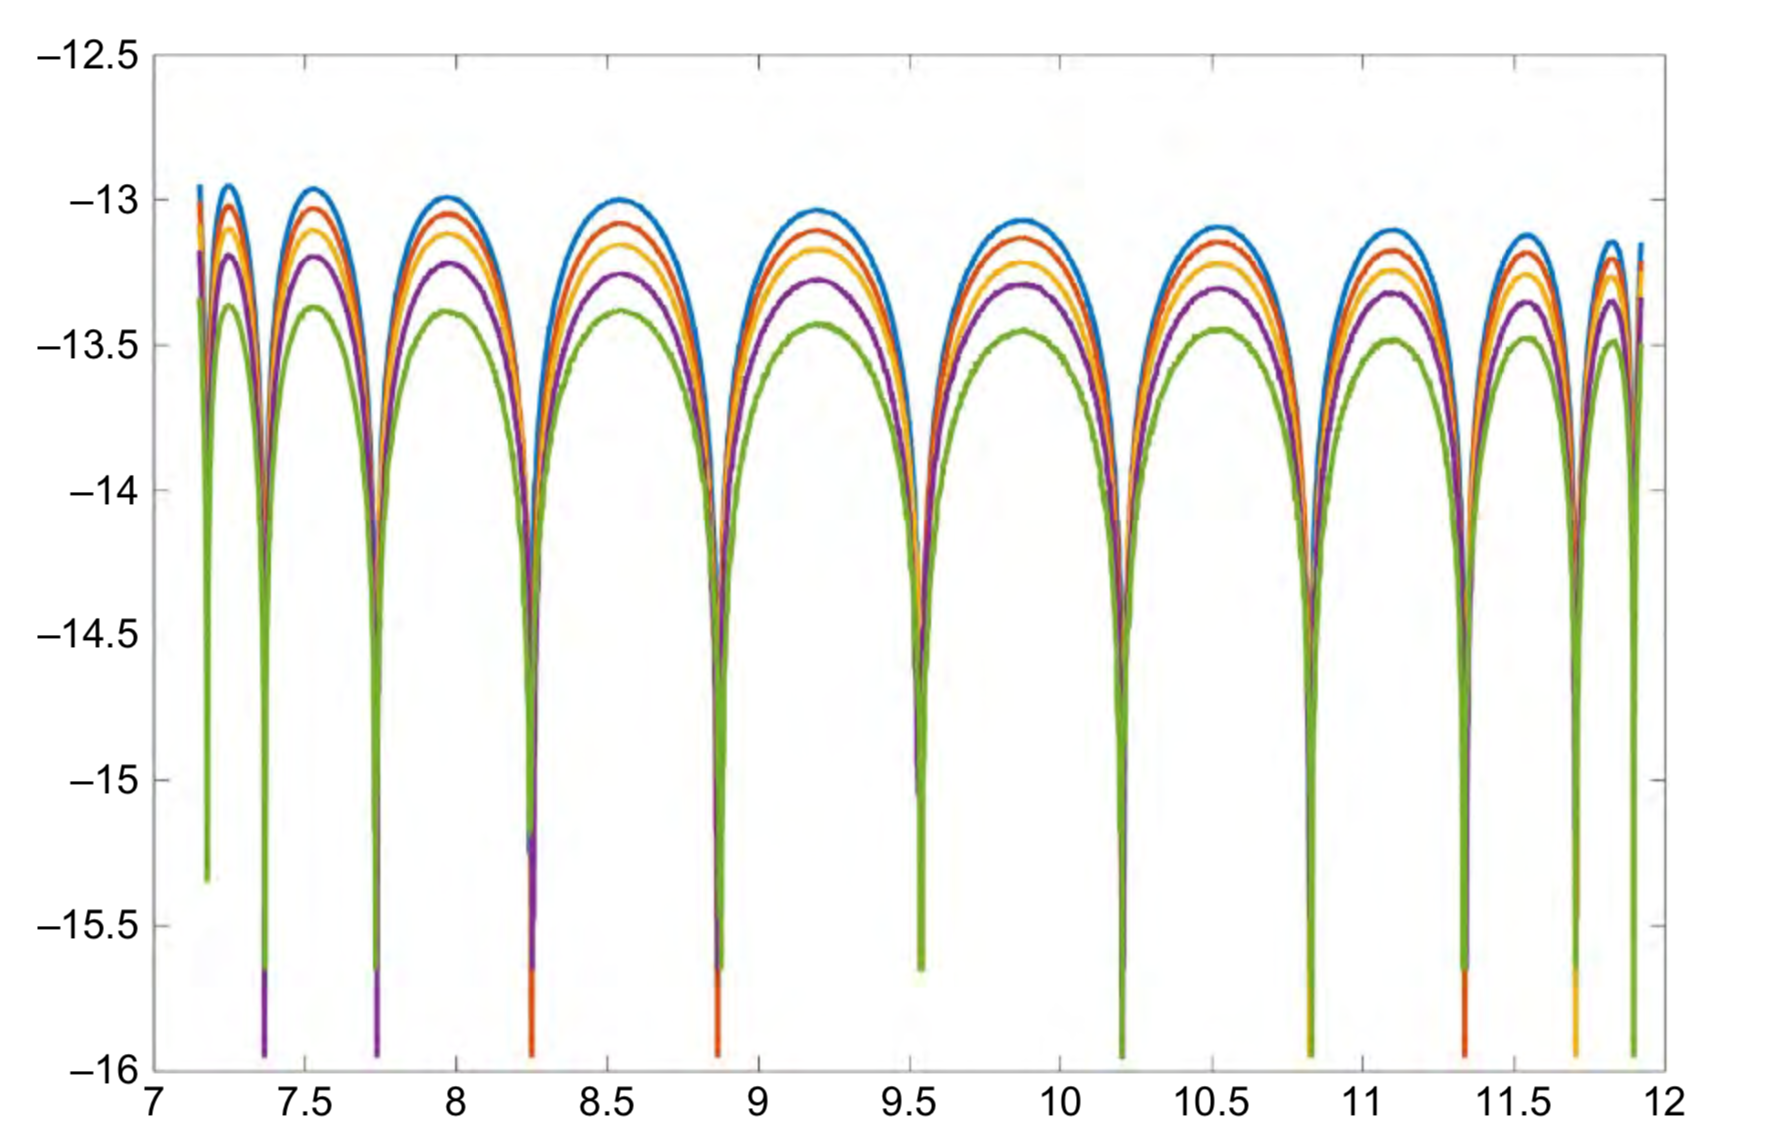
\includegraphics[width=12cm]{./Figures/20180328-eee-ncgt-analysis}
  \label{fig:error-eee-log}
%
%  \small{Source: PBOC.}
\end{figure}

图\ref{fig:error-eee-comp}列出了几种不同近似方法下$\log_{10} EEE\left(k_{t}, z_{t} \right)$的比较,来自\citep{Aruoba:2006cz}的随机NCGT模型(与本文第\ref{sec:pj-example-solution-dsge}节的模型基本类似,除了几处餐厨校准和生产率$z_{t}$的处理)。两张图均设$z_{t}=0$,
以及资本沿着稳态值$k=23.14$的 $70\% $和$130\%$之间截取$\log_{10}EEE$展开分析。
\begin{figure}
\centering
\caption{欧拉等式误差检测的比较}
\label{fig:error-eee-comp}
\subfigure[扰动法]{
\label{fig:error-eee-comp-pt}
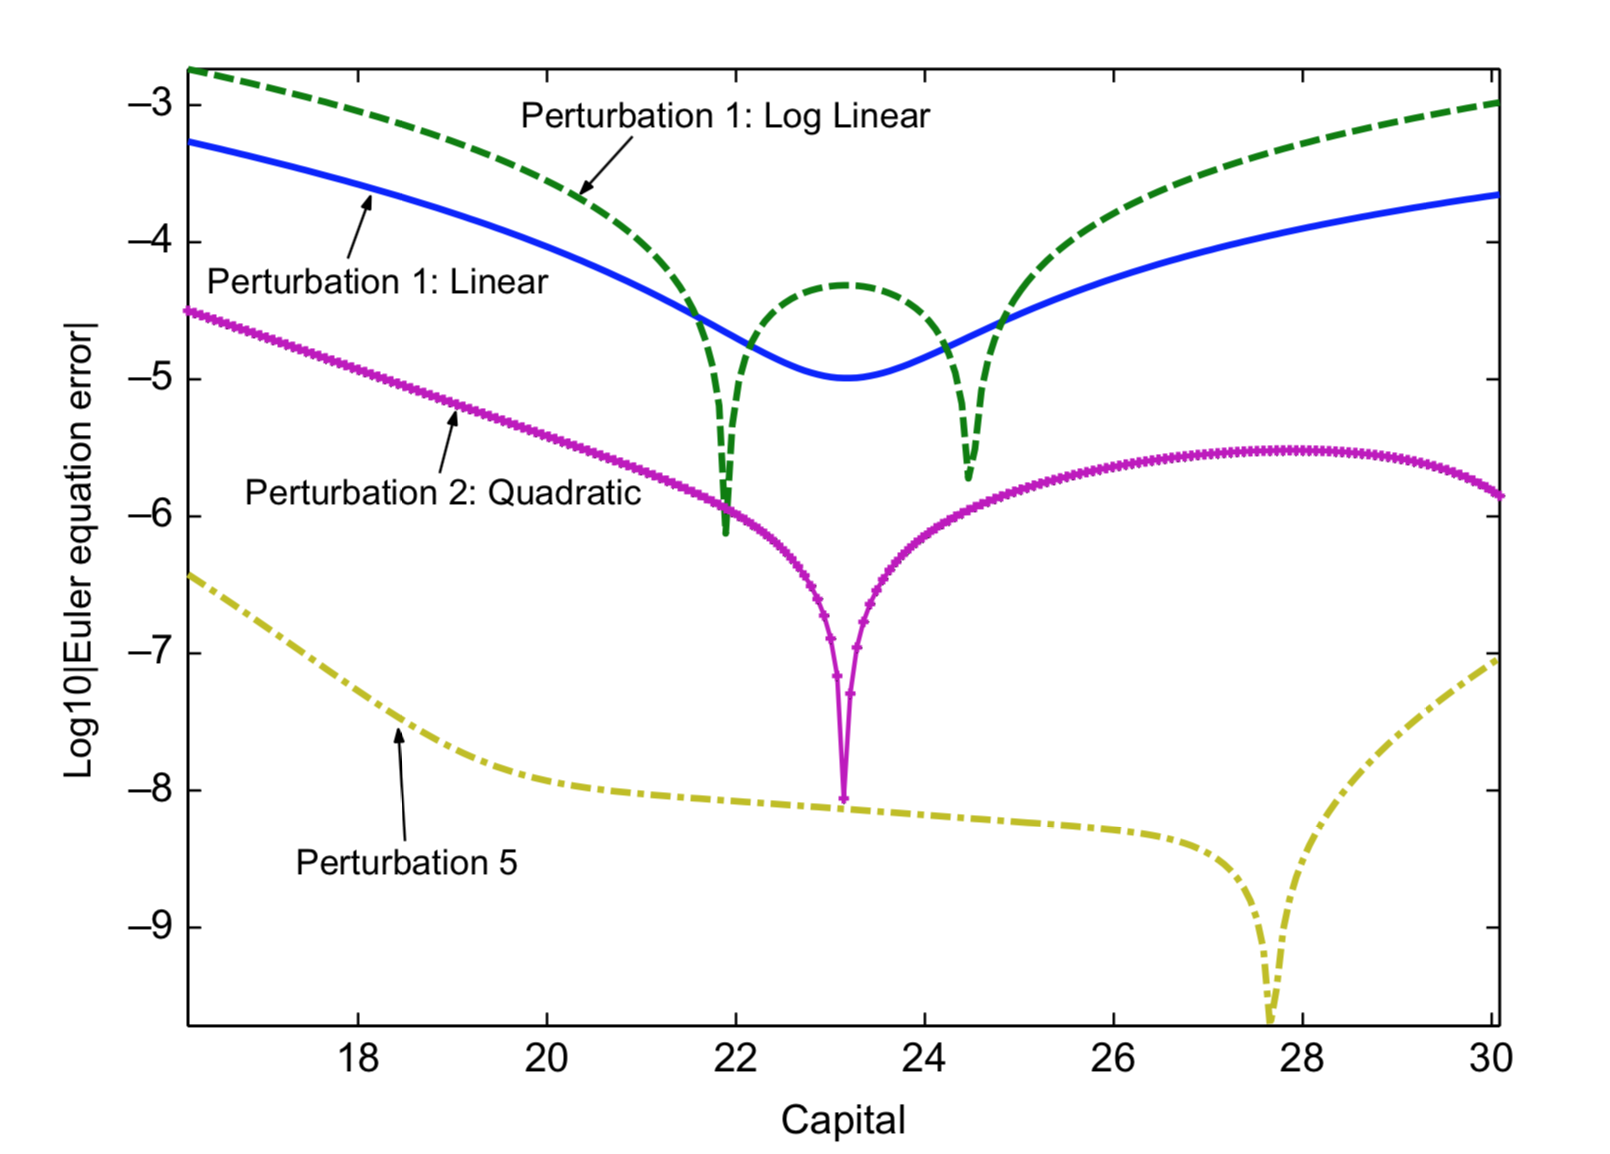
\includegraphics[width=0.8\columnwidth]{./Figures/20180328-eee-comp-pt}
}
\subfigure[投影法]{
\label{fig:error-eee-comp-pj}
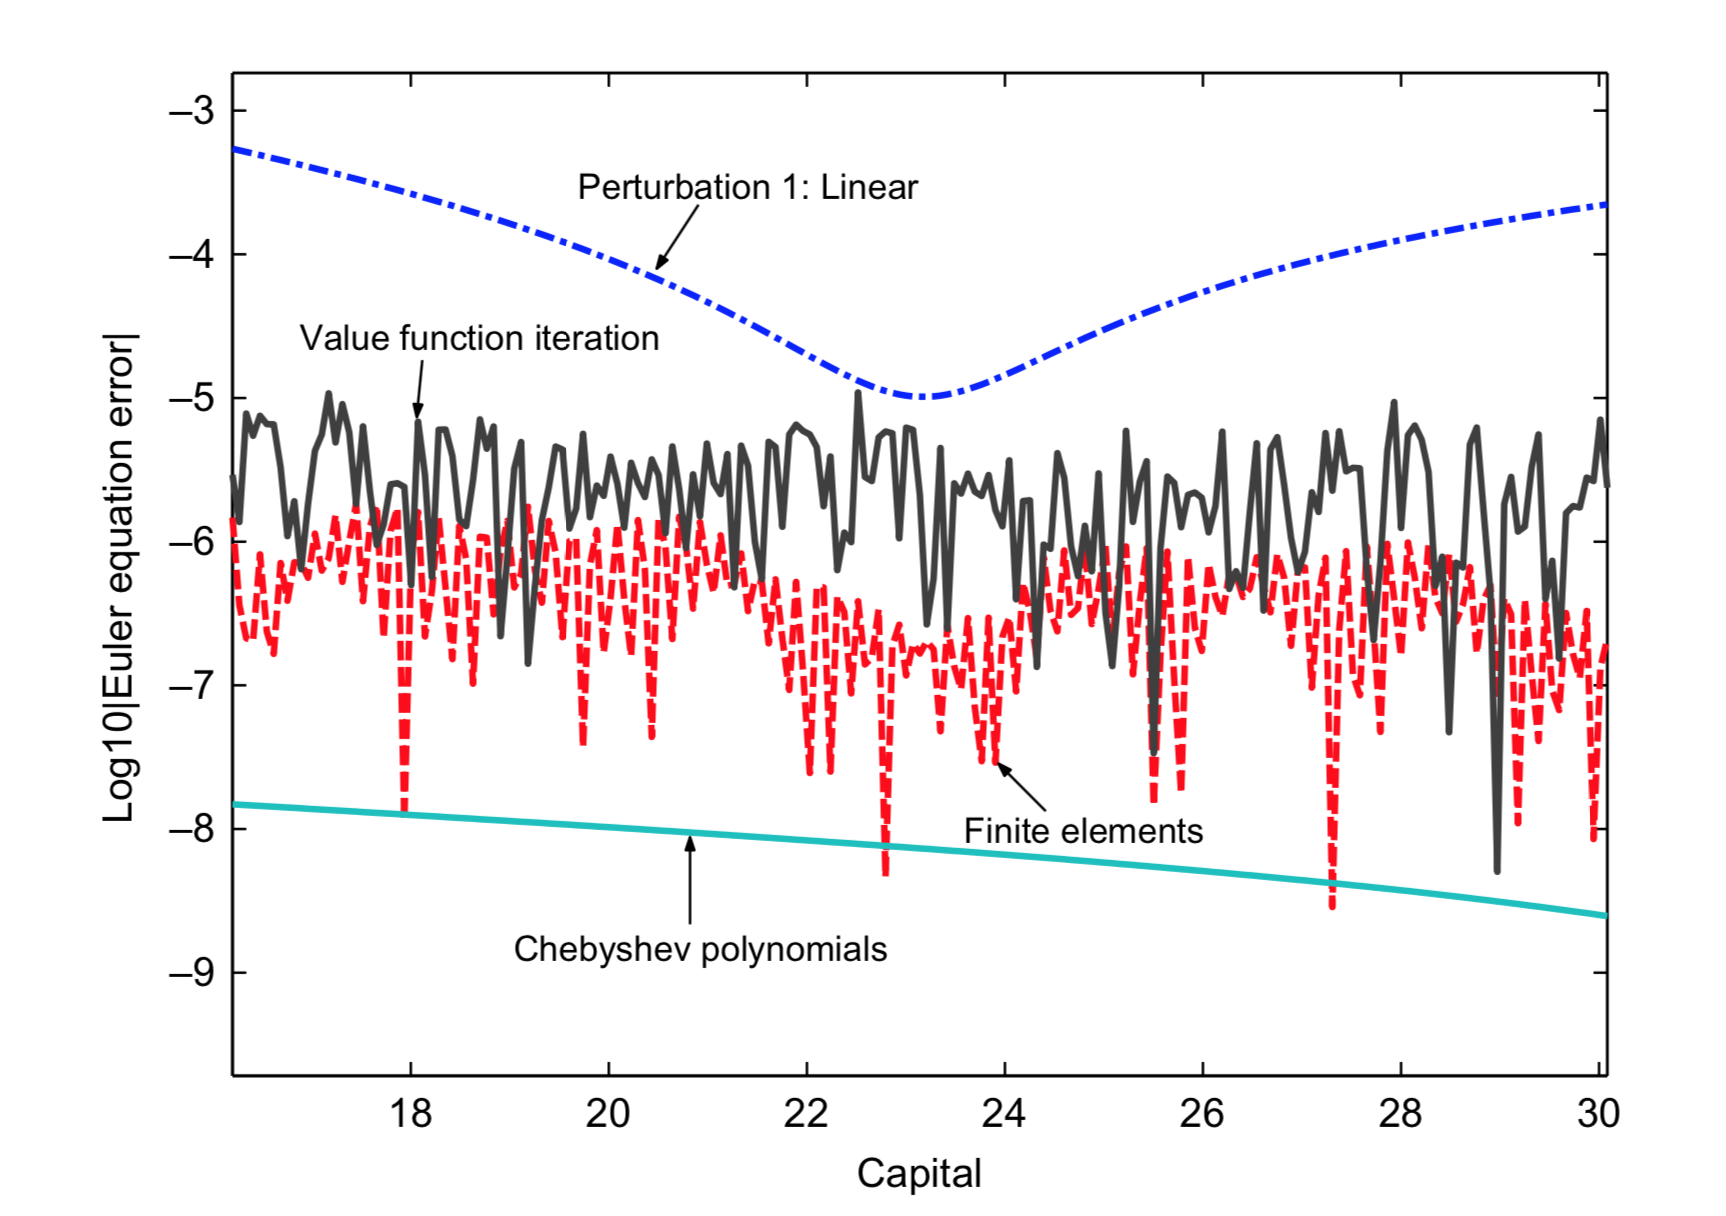
\includegraphics[width=0.8\columnwidth]{./Figures/20180328-eee-comp-pj}
}
\end{figure}

\begin{enumerate}
  \item 图\ref{fig:error-eee-comp-pt}分别画出1阶扰动(对数线性)、1阶扰动(线性)、2阶和5阶扰动的$\log_{10}EEE$。不难看出
\begin{enumerate}
  \item 在稳态点$k=23.14$附近,误差值明显低,越远离稳态点的$k_{t}$取值,对应的误差越大,
  \item 从1阶到2阶近似,精度有明显提升,
  \item 5阶近似的精度很高,并且几乎是全局最优的——即便$k_{t}$取值远离稳态值的30\%以上,精度仍保持在一个较高的水平上。
\end{enumerate}

\item 图\ref{fig:error-eee-comp-pj}分别画出价值方程迭代($25,000 \times 40 = 1,000,000$个网格点,$25,000$和$40$分别表示$k_{t}$和$z_{t}$)、有限元($71$个有限元)、切比雪夫多项式(11个多项式,如第\ref{sec:pj-example-solution-dsge}节模型设定)
的$ \log_{10} EEE$,此外绘出1阶扰动(线性)的误差作为比较。不难看出
\begin{enumerate}
  \item 比起局部的扰动法来,全局性的价值方程迭代法和投影法的精度更高。

  \item 价值方程迭代、有限元和切比雪夫多项式对应的$EEE$较难直观理解,因为他们分别依赖于求解过程中设定的网格点数量、有限元划分、切比雪夫多项式设定。但三者之中,切比雪夫多项式方法提供了最精确的全局解,并且程序运算的时间也是三者中最低的:这与模型设定有关,随机NCGT模型的决策法则总的来说表现良好,非常适合用光谱基方程来做近似。
\end{enumerate}
\end{enumerate}
欧拉方程误差的检测已经成为DSGE模型近似求解过程中判断解法精度的标准检测手段之一,这是由于它所能提供的一系列非常有价值的数据。但需要指出的是,它也存在先天不足,主要表现在很难对近似误差随时间的累积过程作出详细说明。例如,\cite{Santos:2005dz}介绍了如何理解欧拉方程误差对模型近似矩的影响。因此,欧拉方程误差检测可以作为$\chi^{2}$-检测的有益补充,但不能完全替代后者。

\section{误差值的改进}
\label{eq:error-improvement}
在求得近似解的误差后,可以决定是否进一步提高近似解的精度。这涉及到取舍权衡问题:理论上来讲,精度越高越好,然而实际操作过程中,追求精度的提升往往意味着更长的编程时间,更久的程序运行时间。以图\ref{fig:error-eee-comp-pj}为例,在用有限元法作近似求解的过程中,我们可以使用一些现代的科学计算库比如GNU多重精度运算库(GNU Multiple Precision Arithmetic Library, GMP),来在硬件(CPU、内存等)和时间允许的范围内,追求给定精度的计算。在研究过程中做灵活掌握:先从最简单的近似方法入手,如果计算精度未达到要求,就进一步调整近似算法。

如果研究目标对精度没有特别高的要求,那么可以做如下选择
\begin{enumerate}
  \item 若采用扰动法,可以进一步提高扰动的阶数。
  \item 若采用投影法,克增加基方程中元素的数量。
  \item 此外也可以做变量变换或改变求解方法,以使得代求解系统进一步线性化。
\end{enumerate}
